\begin{figure}
    \centering
    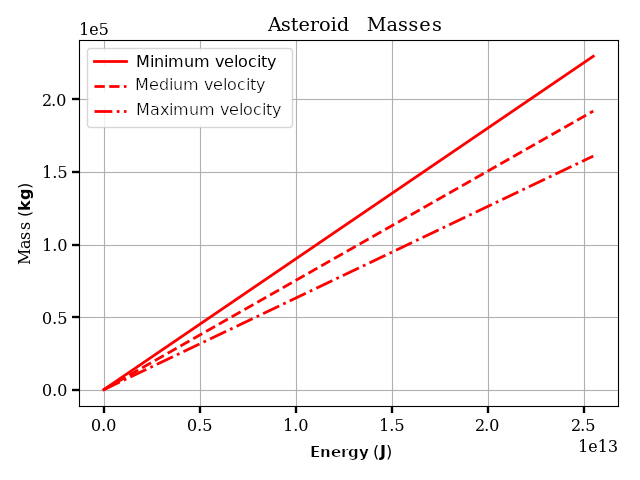
\includegraphics[width=\linewidth]{../figures/Energy_vs_Mass-fireballs_en}
    \caption{Bolides mass derived from Fragment Cloud Model. We used three assumptions about the bolide velocity: Minimum velocity $(\sim \SI{15}{km.s^{-1}})$, Medium velocity $(\sim \SI{16}{km.s^{-1}})$ and maximum velocity $(\sim \SI{18}{km.s^{-1}})$. This values are based on the available data of USG sample (see table \ref{tab:table-meteors-2})}
    \label{fig:energy-mass}
\end{figure}

Once the estimated the bolides energy, we are capable to estimate other bolides parameters, such as the mass. For that we used a Fragment Cloud Model \citep{Wheeler:2017}. To obtain the bolide mass, we must have previous knowledge of its velocity. Based on the few events of the USG sample where we could extract the velocity (see table \ref{tab:table-meteors-2}), we tried three models of bolides mass as a function of its releasing energy: the low velocity model, which assumes a velocity of $\sim \SI{15}{km.s{^-1}}$, medium velocty $v \sim \SI{16}{km.s{^-1}}$ and high velocity $v \sim \SI{18}{km.s{^-1}}$. The resultant masses can be seen in figure \ref{fig:energy-mass}. For the rest of the sample we need to assume that the bolides velocity is within this range or close enough in order to get a reasonable estimation of its mass.